% Synapse Parameters Table
% Required packages: \usepackage{amsmath}, \usepackage{graphicx}, \usepackage{multirow}
\begin{table}[h!]
\centering
\renewcommand{\arraystretch}{1.4}
\resizebox{\textwidth}{!}{%
\begin{tabular}{llccccccc}
\toprule
\multirow{2}{*}{\textbf{Pré-sináptico}} & \multirow{2}{*}{\textbf{Pós-sináptico}} & \multirow{2}{*}{\textbf{Conexão}} & $P$ & \textbf{$g$} & \textbf{$\tau_d$} & \textbf{$\tau_r$} & \textbf{$\tau_f$} & \textbf{$U$} \\
 & & & (\%) & (nS) & (ms) & (ms) & (ms) &  \\
\midrule
$\vcenter{\hbox{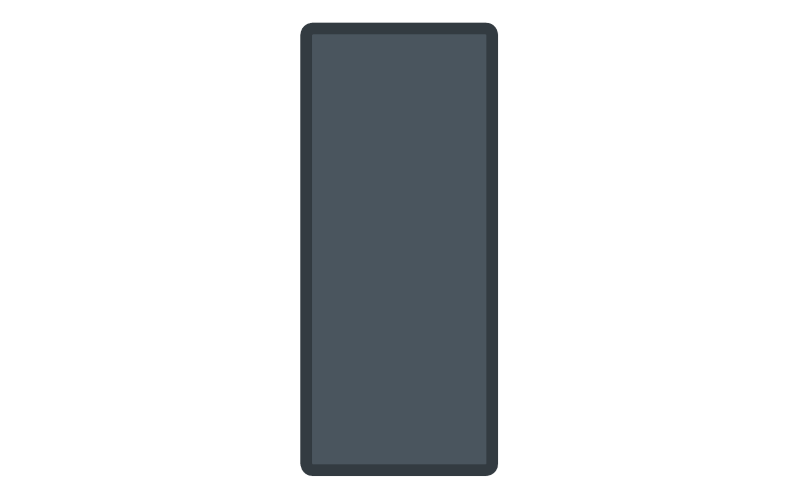
\includegraphics[height=1.5em]{figuras/neurônios/pp.png}}}$ Córtex Entorrinal & $\vcenter{\hbox{
\includegraphics[height=1.5em]{figuras/neurônios/mgc.png}}}$ Granular madura & Aleatória & 8 & 1.825 & 5.333 & 266.239 & 18.714 & 0.27 \\
$\vcenter{\hbox{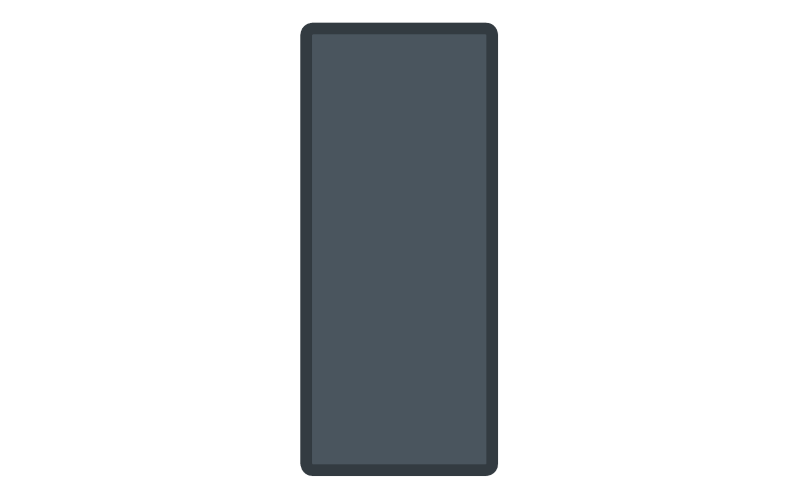
\includegraphics[height=1.5em]{figuras/neurônios/pp.png}}}$ Córtex Entorrinal & $\vcenter{\hbox{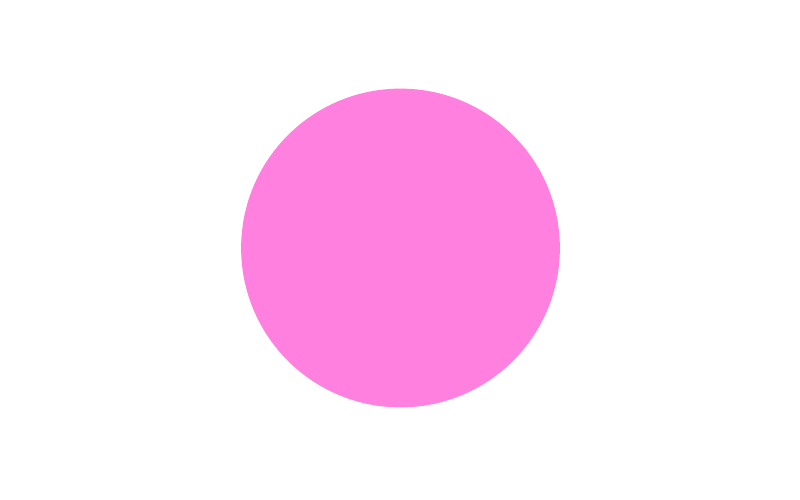
\includegraphics[height=1.5em]{figuras/neurônios/igc.png}}}$ Granular imatura & Aleatória & 8 & 1.825 & 5.333 & 266.239 & 18.714 & 0.27 \\
$\vcenter{\hbox{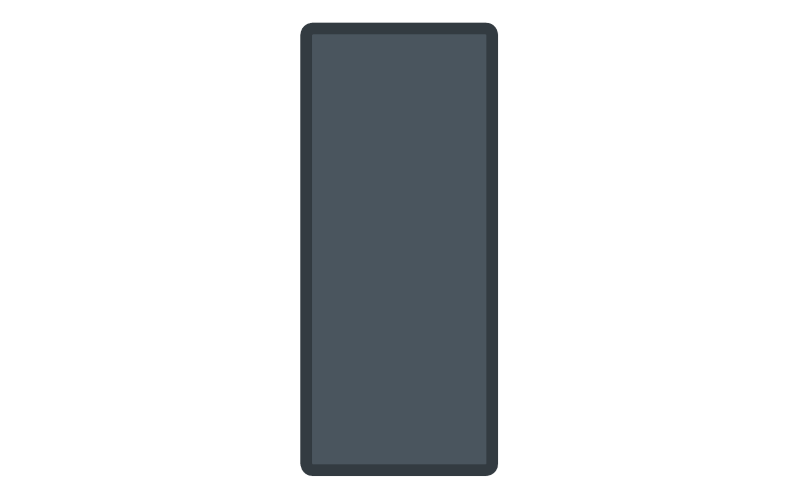
\includegraphics[height=1.5em]{figuras/neurônios/pp.png}}}$ Córtex Entorrinal & $\vcenter{\hbox{
\includegraphics[height=1.5em]{figuras/neurônios/mc.png}}}$ Musgosa & Aleatória & 20 & 1.422 & 4.671 & 319.835 & 57.766 & 0.204 \\
$\vcenter{\hbox{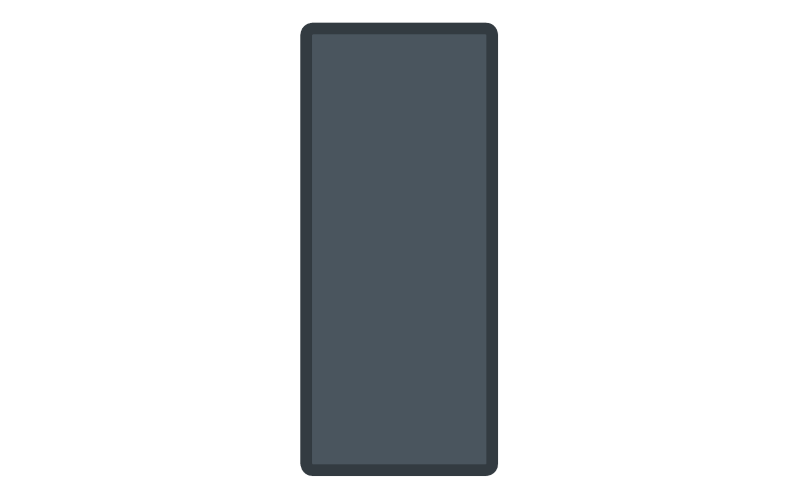
\includegraphics[height=1.5em]{figuras/neurônios/pp.png}}}$ Córtex Entorrinal & $\vcenter{\hbox{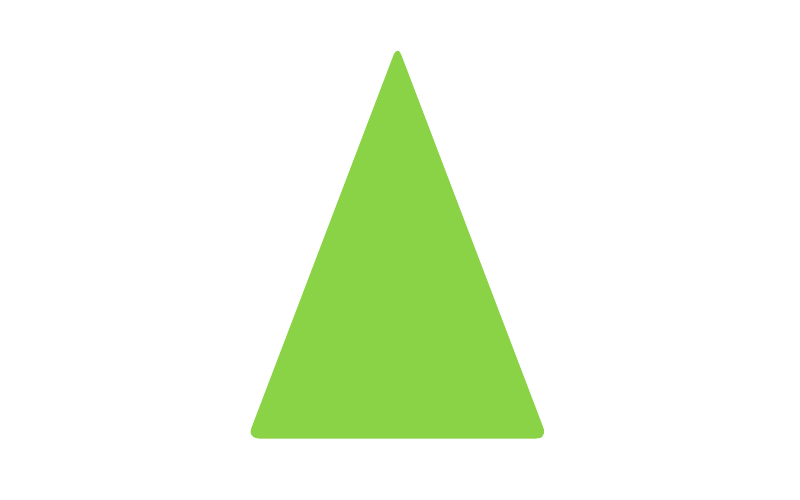
\includegraphics[height=1.5em]{figuras/neurônios/bc.png}}}$ Em cesto & Aleatória & 20 & 1.406 & 3.849 & 144.415 & 48.2 & 0.214 \\
$\vcenter{\hbox{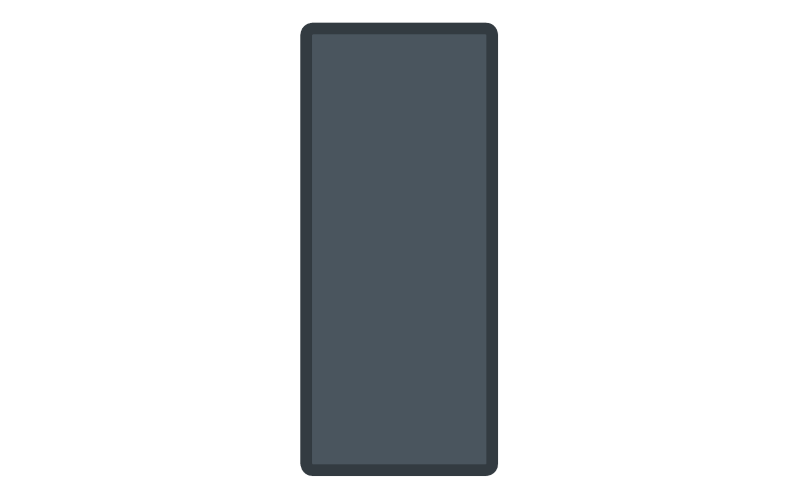
\includegraphics[height=1.5em]{figuras/neurônios/pp.png}}}$ Córtex Entorrinal & $\vcenter{\hbox{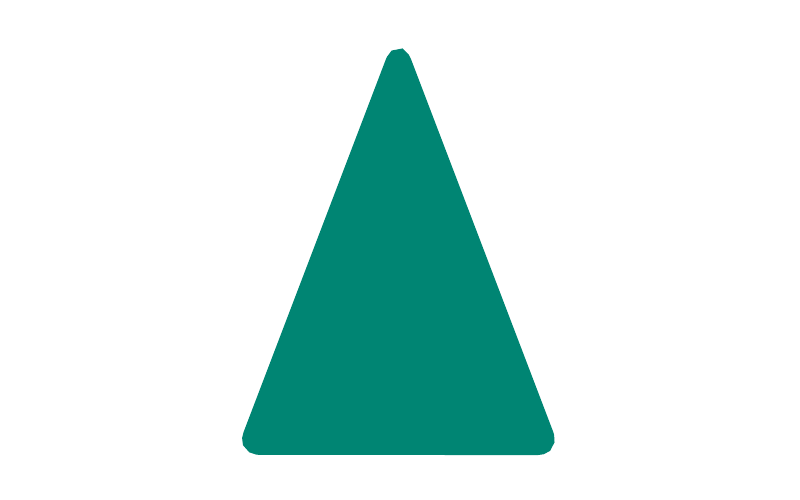
\includegraphics[height=1.5em]{figuras/neurônios/pca3.png}}}$ Piramidal do CA3 & Aleatória & 4 & 1.065 & 6.55 & 258.318 & 53.478 & 0.184 \\
$\vcenter{\hbox{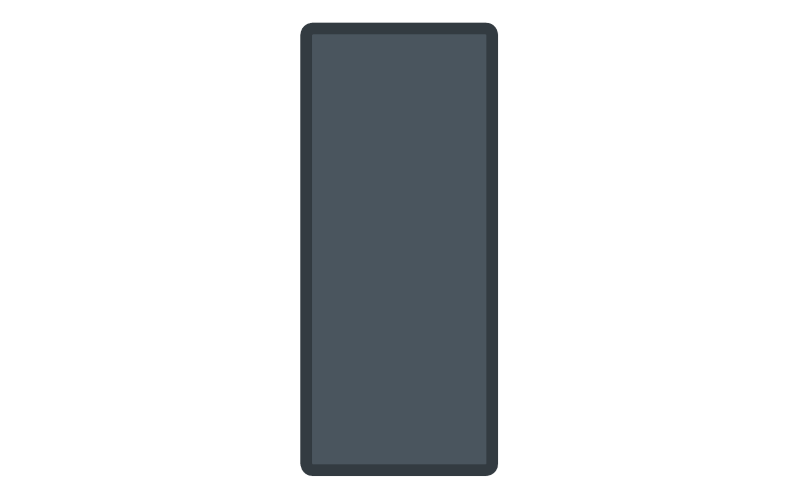
\includegraphics[height=1.5em]{figuras/neurônios/pp.png}}}$ Córtex Entorrinal & $\vcenter{\hbox{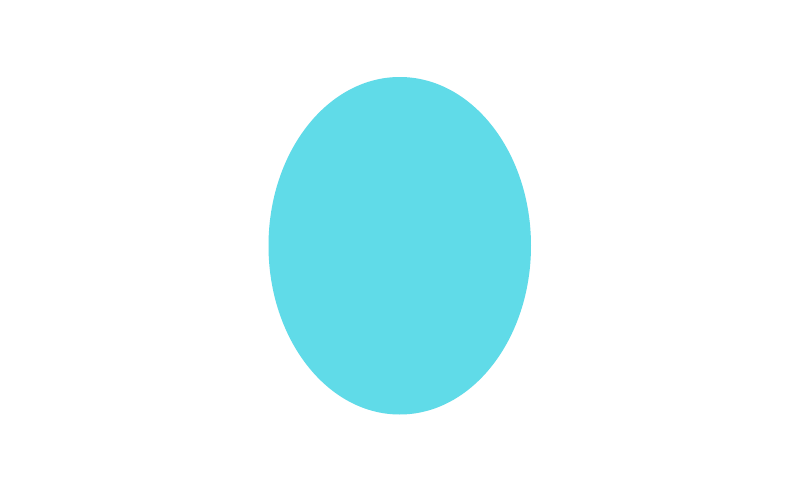
\includegraphics[height=1.5em]{figuras/neurônios/ica3.png}}}$ Inibitória do CA3 & Aleatória & 20 & 1.556 & 3.602 & 457.468 & 35.904 & 0.21 \\
$\vcenter{\hbox{
\includegraphics[height=1.5em]{figuras/neurônios/mgc.png}}}$ Granular madura & $\vcenter{\hbox{
\includegraphics[height=1.5em]{figuras/neurônios/mc.png}}}$ Musgosa & Lamelar & 20 & 1.713 & 5.347 & 428.583 & 73.479 & 0.151 \\
$\vcenter{\hbox{
\includegraphics[height=1.5em]{figuras/neurônios/mgc.png}}}$ Granular madura & $\vcenter{\hbox{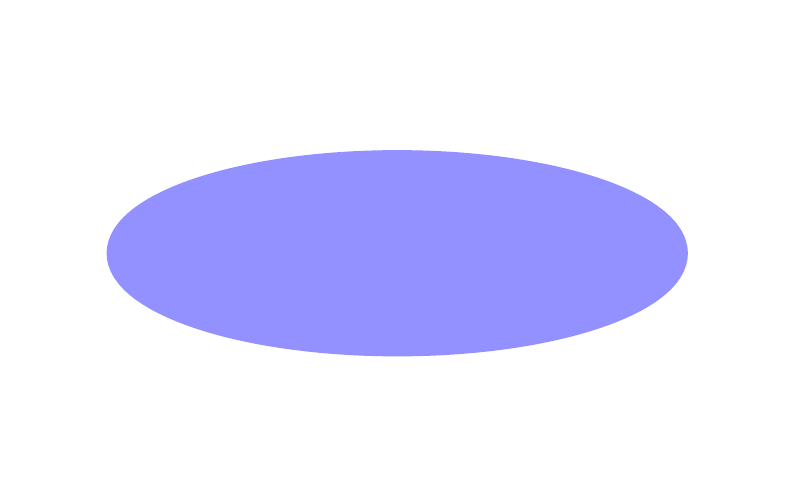
\includegraphics[height=1.5em]{figuras/neurônios/hipp.png}}}$ HIPP & Aleatória & 10 & 1.305 & 5.181 & 462.814 & 48.986 & 0.15 \\
$\vcenter{\hbox{
\includegraphics[height=1.5em]{figuras/neurônios/mgc.png}}}$ Granular madura & $\vcenter{\hbox{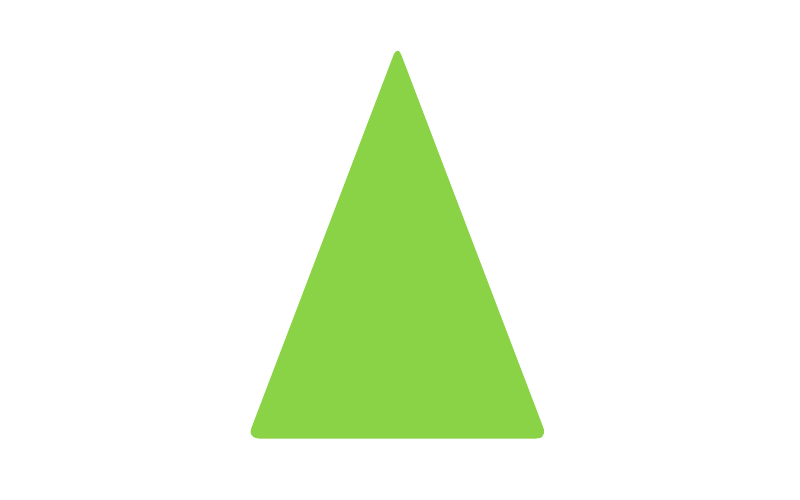
\includegraphics[height=1.5em]{figuras/neurônios/bc.png}}}$ Em cesto & Lamelar & 100 & 1.458 & 3.566 & 151.265 & 62.278 & 0.197 \\
$\vcenter{\hbox{
\includegraphics[height=1.5em]{figuras/neurônios/mgc.png}}}$ Granular madura & $\vcenter{\hbox{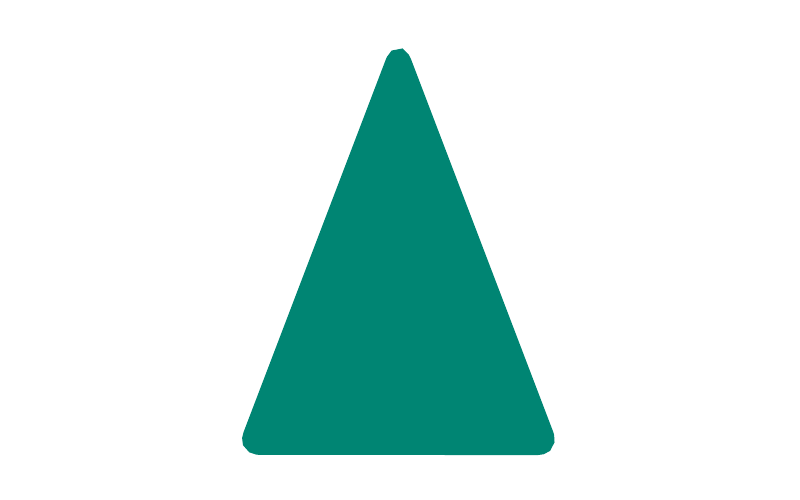
\includegraphics[height=1.5em]{figuras/neurônios/pca3.png}}}$ Piramidal do CA3 & Lamelar & 60 & 1.384 & 6.657 & 278.286 & 78.584 & 0.155 \\
$\vcenter{\hbox{
\includegraphics[height=1.5em]{figuras/neurônios/mgc.png}}}$ Granular madura & $\vcenter{\hbox{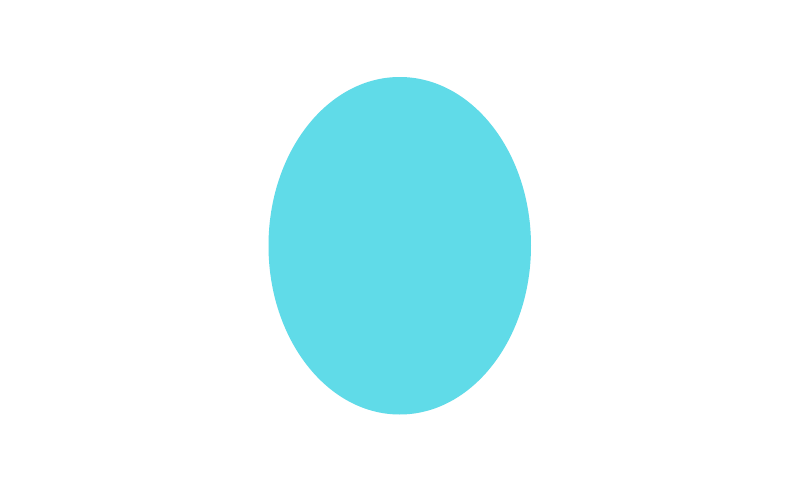
\includegraphics[height=1.5em]{figuras/neurônios/ica3.png}}}$ Inibitória do CA3 & Lamelar & 100 & 1.625 & 3.915 & 518.934 & 43.274 & 0.176 \\
$\vcenter{\hbox{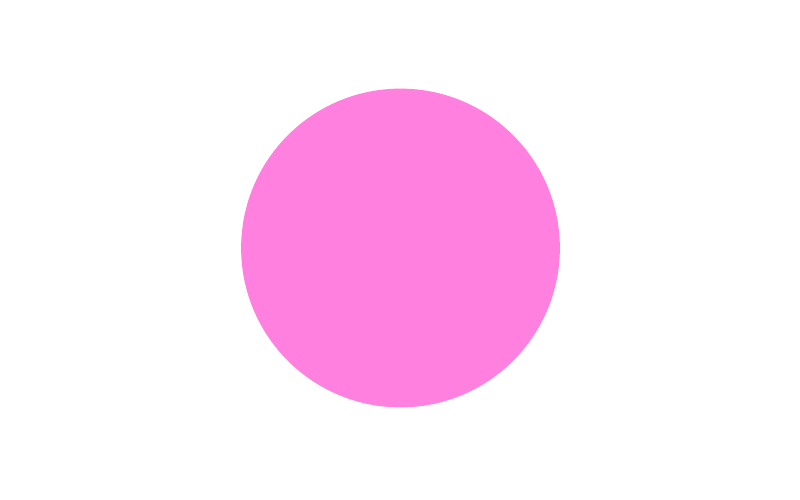
\includegraphics[height=1.5em]{figuras/neurônios/igc.png}}}$ Granular imatura & $\vcenter{\hbox{
\includegraphics[height=1.5em]{figuras/neurônios/mc.png}}}$ Musgosa & Lamelar & 20 & 1.713 & 5.347 & 428.583 & 73.479 & 0.151 \\
$\vcenter{\hbox{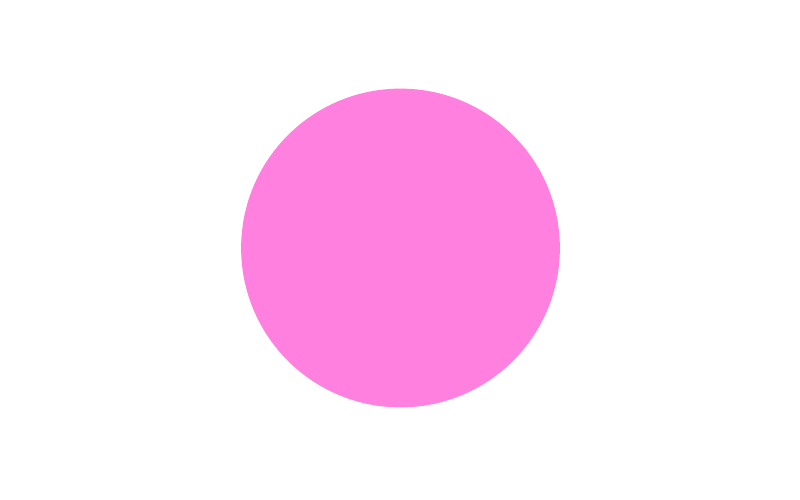
\includegraphics[height=1.5em]{figuras/neurônios/igc.png}}}$ Granular imatura & $\vcenter{\hbox{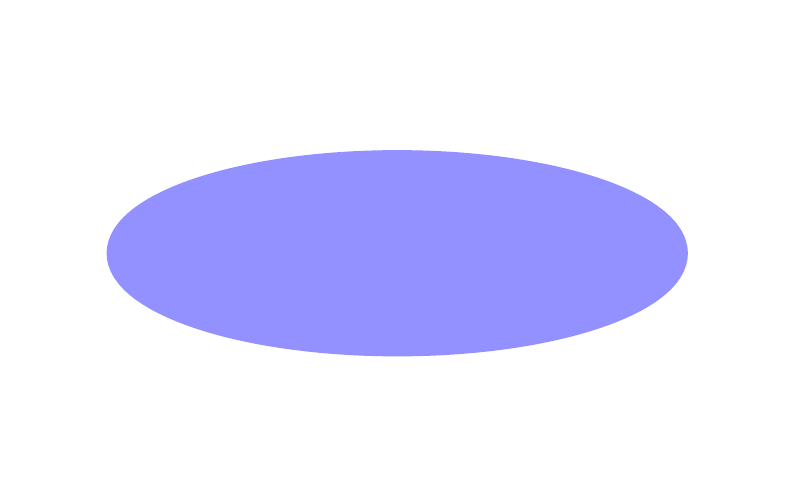
\includegraphics[height=1.5em]{figuras/neurônios/hipp.png}}}$ HIPP & Aleatória & 10 & 1.305 & 5.181 & 462.814 & 48.986 & 0.15 \\
$\vcenter{\hbox{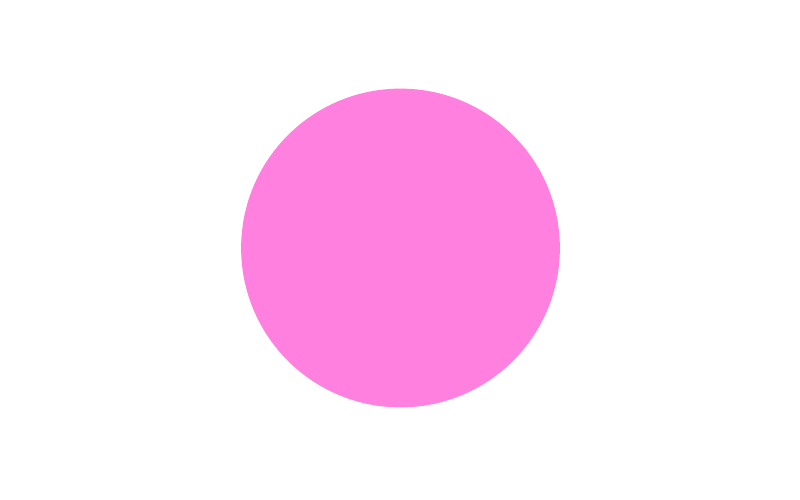
\includegraphics[height=1.5em]{figuras/neurônios/igc.png}}}$ Granular imatura & $\vcenter{\hbox{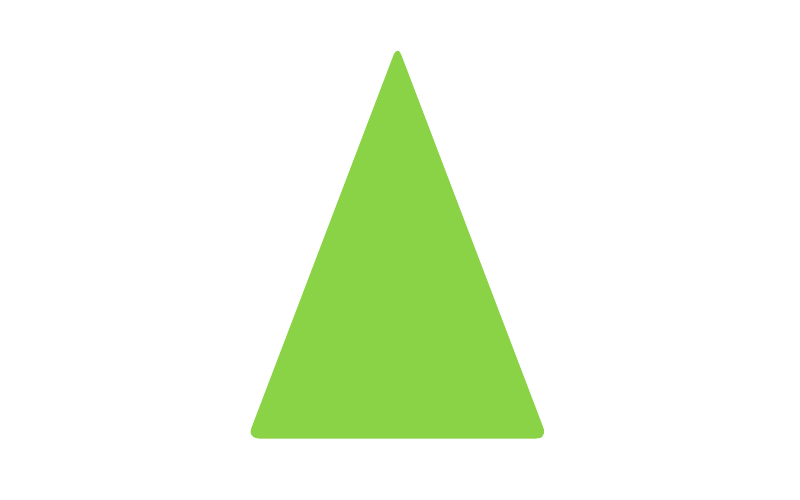
\includegraphics[height=1.5em]{figuras/neurônios/bc.png}}}$ Em cesto & Lamelar & 100 & 1.458 & 3.566 & 151.265 & 62.278 & 0.197 \\
$\vcenter{\hbox{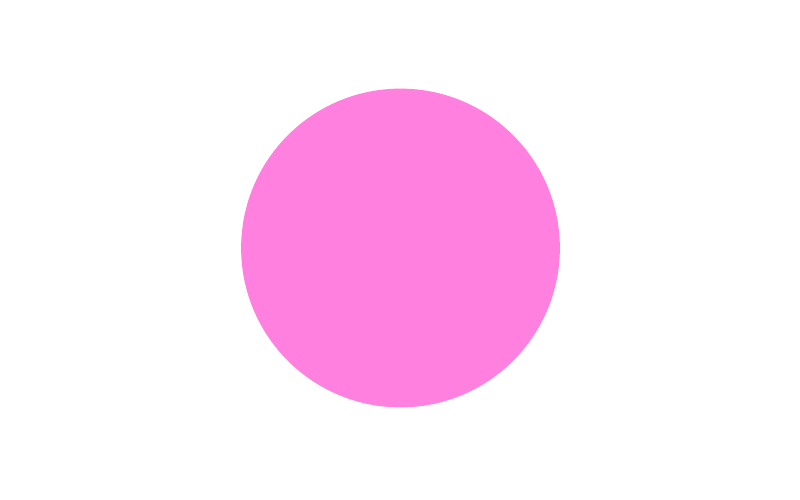
\includegraphics[height=1.5em]{figuras/neurônios/igc.png}}}$ Granular imatura & $\vcenter{\hbox{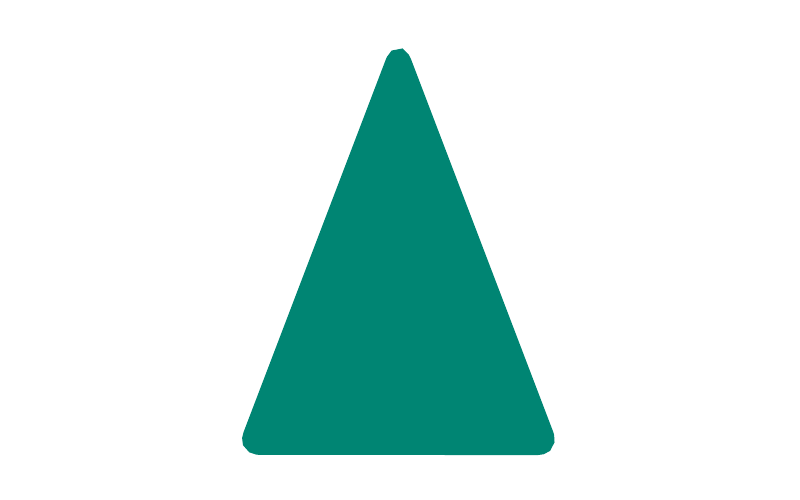
\includegraphics[height=1.5em]{figuras/neurônios/pca3.png}}}$ Piramidal do CA3 & Lamelar & 60 & 1.384 & 6.657 & 278.286 & 78.584 & 0.155 \\
$\vcenter{\hbox{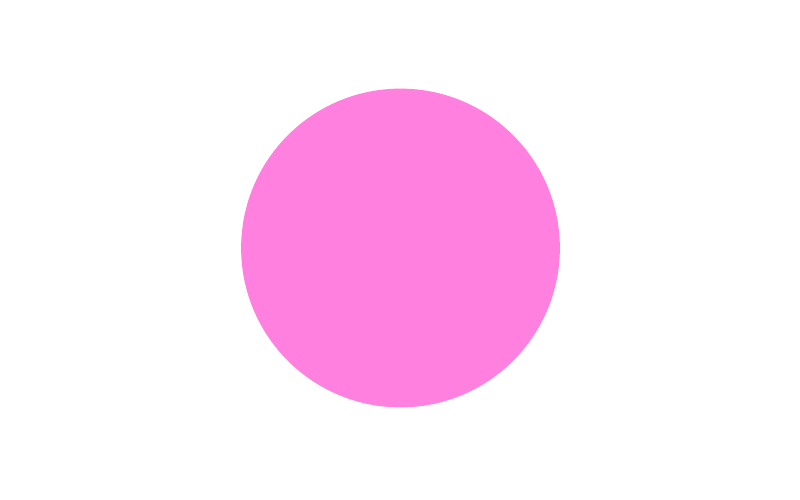
\includegraphics[height=1.5em]{figuras/neurônios/igc.png}}}$ Granular imatura & $\vcenter{\hbox{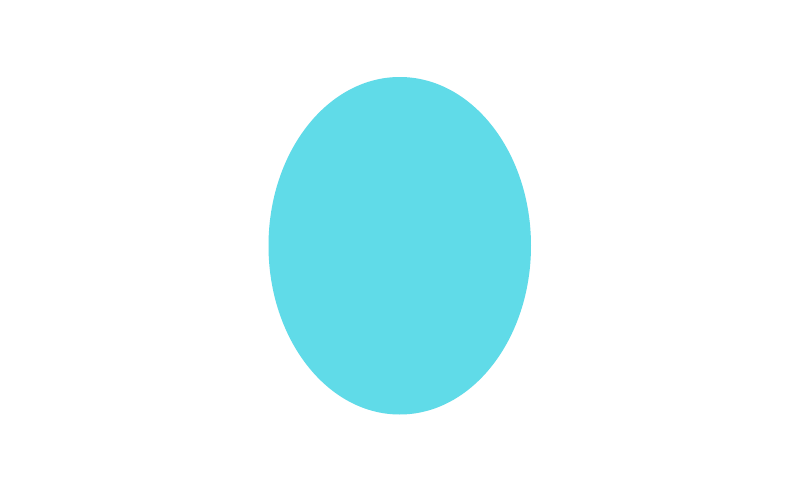
\includegraphics[height=1.5em]{figuras/neurônios/ica3.png}}}$ Inibitória do CA3 & Lamelar & 100 & 1.625 & 3.915 & 518.934 & 43.274 & 0.176 \\
$\vcenter{\hbox{
\includegraphics[height=1.5em]{figuras/neurônios/mc.png}}}$ Musgosa & $\vcenter{\hbox{
\includegraphics[height=1.5em]{figuras/neurônios/mgc.png}}}$ Granular madura & Interlamelar & 0.2 & 2.394 & 5.357 & 166.162 & 20.224 & 0.304 \\
$\vcenter{\hbox{
\includegraphics[height=1.5em]{figuras/neurônios/mc.png}}}$ Musgosa & $\vcenter{\hbox{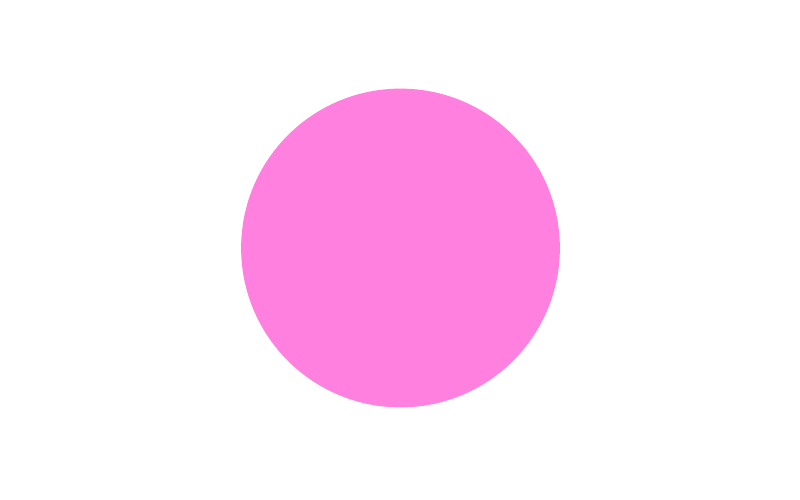
\includegraphics[height=1.5em]{figuras/neurônios/igc.png}}}$ Granular imatura & Interlamelar & 0.2 & 2.394 & 5.357 & 166.162 & 20.224 & 0.304 \\
$\vcenter{\hbox{
\includegraphics[height=1.5em]{figuras/neurônios/mc.png}}}$ Musgosa & $\vcenter{\hbox{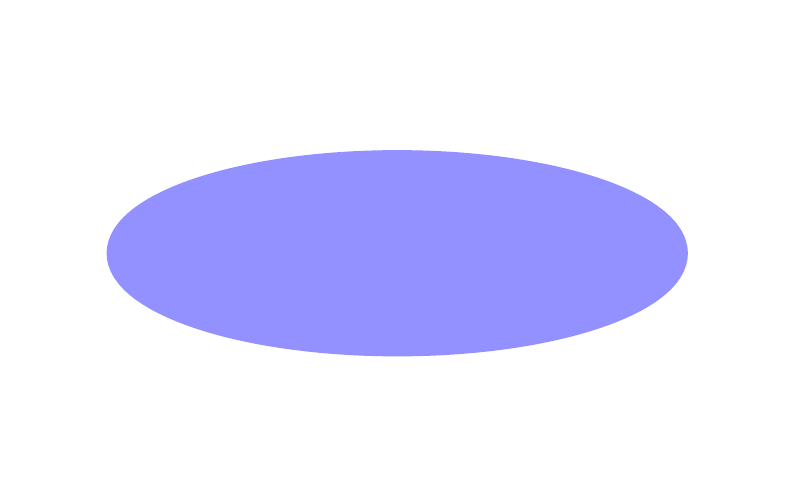
\includegraphics[height=1.5em]{figuras/neurônios/hipp.png}}}$ HIPP & Interlamelar & 100 & 1.376 & 4.824 & 358.431 & 54.872 & 0.181 \\
$\vcenter{\hbox{
\includegraphics[height=1.5em]{figuras/neurônios/mc.png}}}$ Musgosa & $\vcenter{\hbox{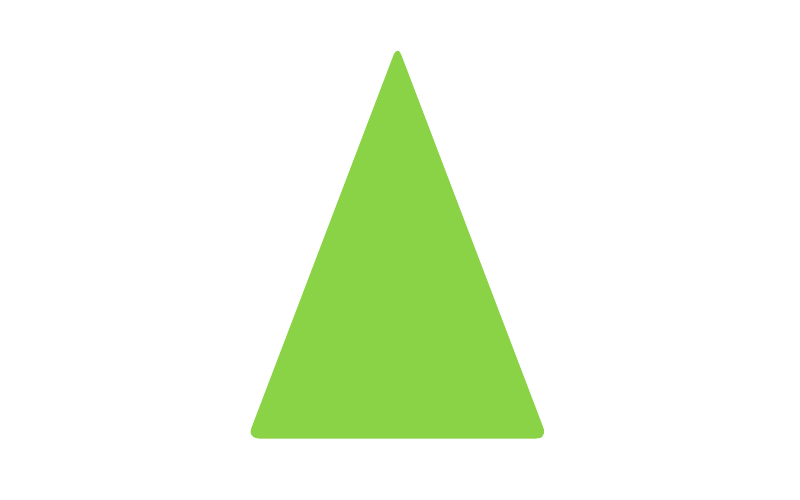
\includegraphics[height=1.5em]{figuras/neurônios/bc.png}}}$ Em cesto & Interlamelar & 100 & 1.996 & 3.396 & 117.365 & 69.316 & 0.255 \\
$\vcenter{\hbox{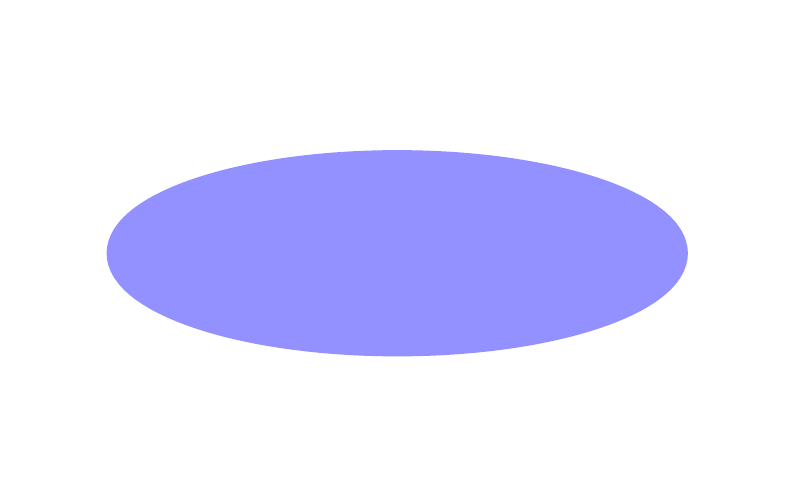
\includegraphics[height=1.5em]{figuras/neurônios/hipp.png}}}$ HIPP & $\vcenter{\hbox{
\includegraphics[height=1.5em]{figuras/neurônios/mgc.png}}}$ Granular madura & Aleatória & 20 & 2.002 & 8.935 & 559.143 & 8.396 & 0.278 \\
$\vcenter{\hbox{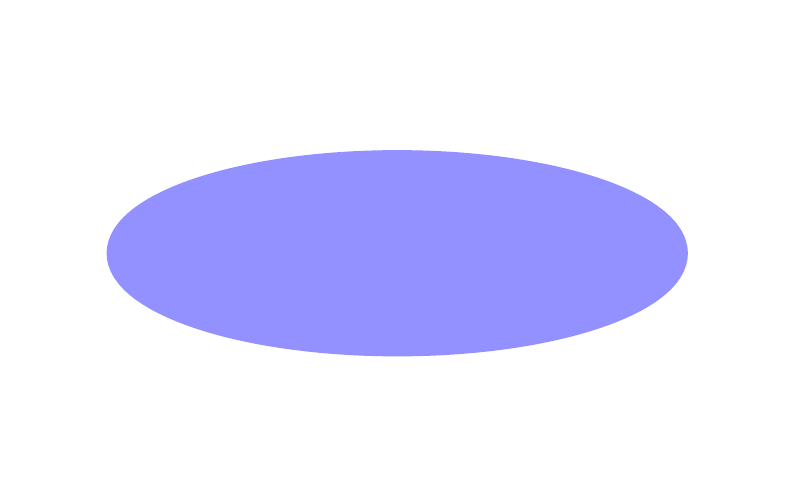
\includegraphics[height=1.5em]{figuras/neurônios/hipp.png}}}$ HIPP & $\vcenter{\hbox{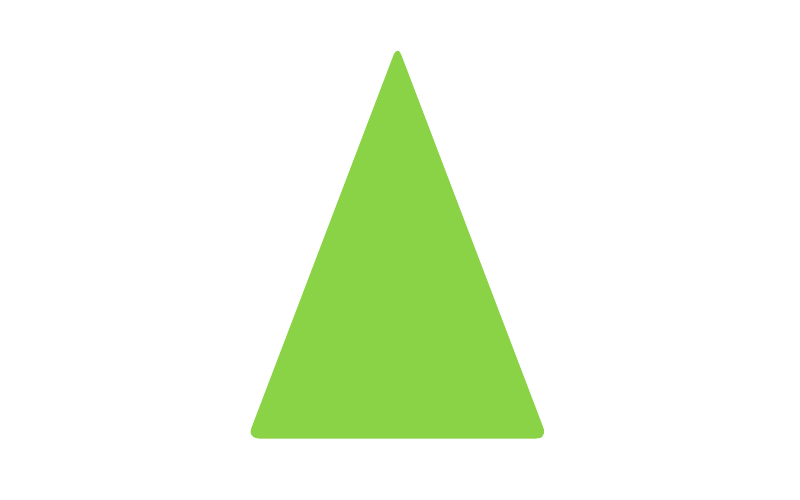
\includegraphics[height=1.5em]{figuras/neurônios/bc.png}}}$ Em cesto & Aleatória & 2 & 1.709 & 5.982 & 367.198 & 15.292 & 0.221 \\
$\vcenter{\hbox{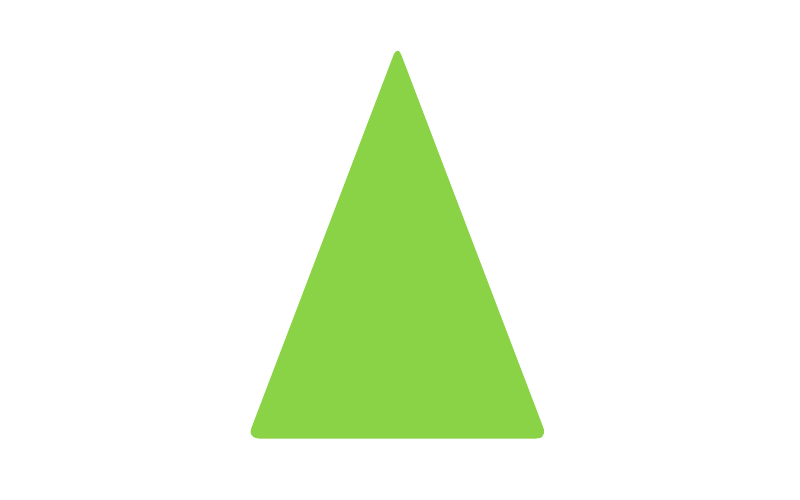
\includegraphics[height=1.5em]{figuras/neurônios/bc.png}}}$ Em cesto & $\vcenter{\hbox{
\includegraphics[height=1.5em]{figuras/neurônios/mgc.png}}}$ Granular madura & Lamelar & 100 & 2.451 & 6.543 & 433.876 & 6.347 & 0.332 \\
$\vcenter{\hbox{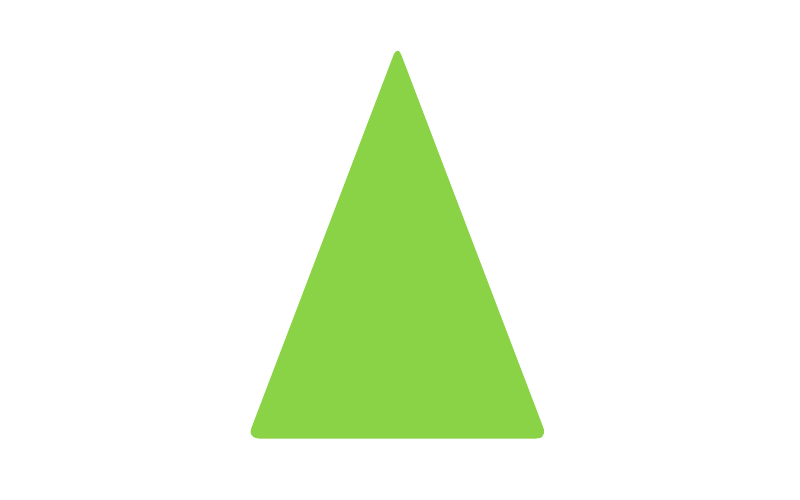
\includegraphics[height=1.5em]{figuras/neurônios/bc.png}}}$ Em cesto & $\vcenter{\hbox{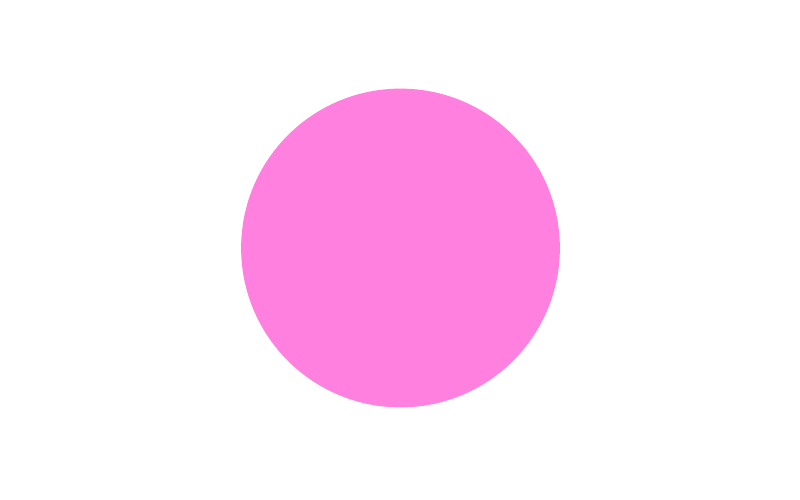
\includegraphics[height=1.5em]{figuras/neurônios/igc.png}}}$ Granular imatura & Lamelar & 100 & 2.451 & 6.543 & 433.876 & 6.347 & 0.332 \\
$\vcenter{\hbox{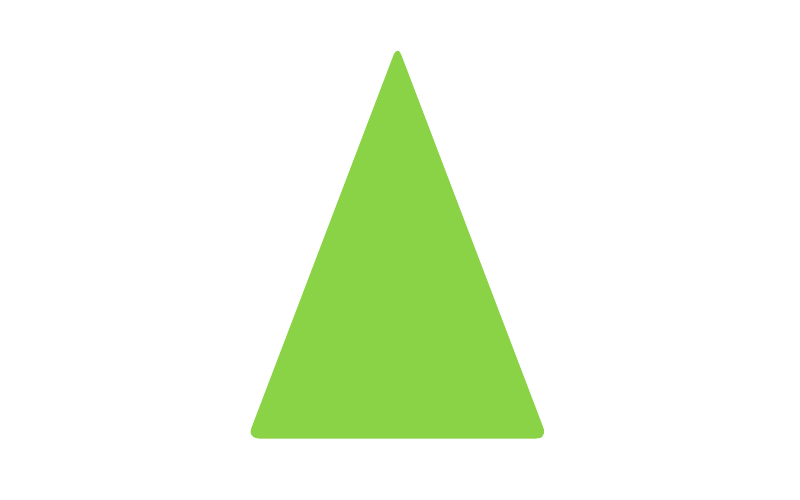
\includegraphics[height=1.5em]{figuras/neurônios/bc.png}}}$ Em cesto & $\vcenter{\hbox{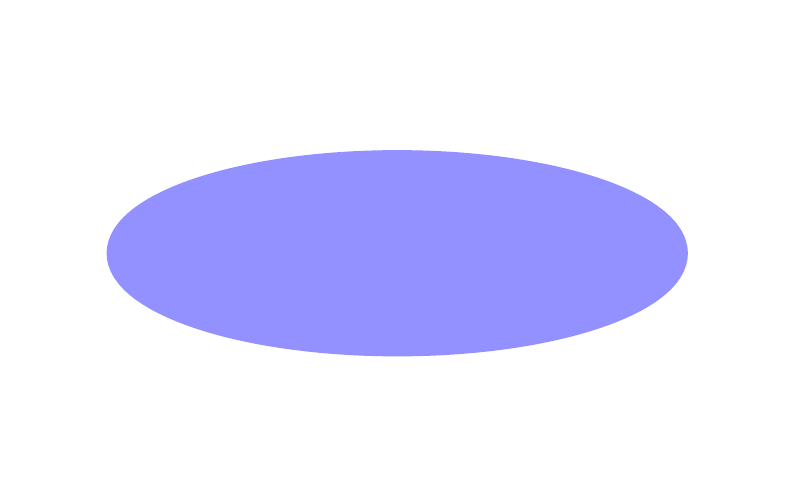
\includegraphics[height=1.5em]{figuras/neurônios/hipp.png}}}$ HIPP & Aleatória & 2 & 1.408 & 6.544 & 534.182 & 8.385 & 0.24 \\
$\vcenter{\hbox{\includegraphics[height=1.5em]{figuras/neurônios/pca3.png}}}$ Piramidal do CA3 & $\vcenter{\hbox{\includegraphics[height=1.5em]{figuras/neurônios/pca3.png}}}$ Piramidal do CA3 & Aleatória & 2 & 0.603 & 9.516 & 278.258 & 27.513 & 0.172 \\
$\vcenter{\hbox{\includegraphics[height=1.5em]{figuras/neurônios/pca3.png}}}$ Piramidal do CA3 & $\vcenter{\hbox{\includegraphics[height=1.5em]{figuras/neurônios/mc.png}}}$ Musgosa & Lamelar & 10 & 2.035 & 4.297 & 359.116 & 40.457 & 0.236 \\
$\vcenter{\hbox{\includegraphics[height=1.5em]{figuras/neurônios/pca3.png}}}$ Piramidal do CA3 & $\vcenter{\hbox{\includegraphics[height=1.5em]{figuras/neurônios/ica3.png}}}$ Inibitória do CA3 & Aleatória & 100 & 1.247 & 4.525 & 525.605 & 23.321 & 0.189 \\
$\vcenter{\hbox{\includegraphics[height=1.5em]{figuras/neurônios/ica3.png}}}$ Inibitória do CA3 & $\vcenter{\hbox{\includegraphics[height=1.5em]{figuras/neurônios/pca3.png}}}$ Piramidal do CA3 & Aleatória & 100 & 1.462 & 7.793 & 416.282 & 20.63 & 0.203 \\
\bottomrule
\end{tabular}}
\caption{Parâmetros das sinapses entre as populações neuronais. Conexões aleatórias ocorrem entre todas as células
              de ambas as populações; conexões lamelares ocorrem entre células da mesma lamela; conexões interlamelares ocorrem
              entre as células de uma lamela com todas as demais. A probabilidade de conexão $P$ diz respeito à porcentagem de
              conexões entre as populações neuronais de acordo com a condição de conexão.}
\label{tab:synapse_params}
\end{table}
